\documentclass{article}

\usepackage[final, nonatbib]{neurips_2024}

\usepackage[utf8]{inputenc} % allow utf-8 input
\usepackage[T1]{fontenc}    % use 8-bit T1 fonts
%\usepackage{hyperref}       % hyperlinks
%\usepackage{url}            % simple URL typesetting
\usepackage{booktabs}       % professional-quality tables
\usepackage{amsfonts}       % blackboard math symbols
\usepackage{nicefrac}       % compact symbols for 1/2, etc.
\usepackage{microtype}      % microtypography
\usepackage{xcolor}         % colors

\usepackage{url}
\def\UrlBreaks{\do\/\do-}
\usepackage{breakurl}
\usepackage[breaklinks]{hyperref}

\usepackage{amsmath}
\usepackage{graphicx}
%\usepackage[colorlinks=true, allcolors=blue]{hyperref}
\usepackage{threeparttable}
%\usepackage[style=ieee,minbibnames=3,natbib=true]{biblatex}
%\addbibresource{sample.bib}
\usepackage{wrapfig}

\usepackage[normalem]{ulem} 
\useunder{\uline}{\ul}{}


\title{Fully Open Source Moxin-LLM Technical Report}

\author{Pu Zhao$^1$, Xuan Shen$^1$, Zhenglun Kong$^2$, Yixin Shen$^{3}$, Sung-En Chang$^1$, \\ \textbf{Timothy Rupprecht$^1$,  Lei Lu$^1$, Enfu Nan$^1$, Changdi Yang$^1$, Yumei He$^4$, }\\ \textbf{Xingchen Xu$^5$, Yu Huang$^6$, Wei Wang$^7$, Yue Chen$^7$, Yong He$^7$, Yanzhi Wang$^{1,8}$} \\
\\$^1$Northeastern University, $^2$Harvard University,  \\ $^3$Cornell University,  $^4$Tulane University,
 $^5$University of Washington,  \\ $^6$Roboraction.ai, $^7$Futurewei Technologies, $^8$AIBAO LLC}



\begin{document}
\maketitle

\begin{abstract}
Recently, Large Language Models (LLMs) have undergone a significant transformation, marked by a rapid rise in both their popularity and capabilities. Leading this evolution are proprietary LLMs like GPT-4 and GPT-o1, which have captured widespread attention in the AI community due to their remarkable performance and versatility. Simultaneously, open-source LLMs, such as LLaMA and Mistral, have made great contributions to the ever-increasing popularity of LLMs due to the ease to customize and deploy the models across diverse applications. Although open-source LLMs present unprecedented opportunities for innovation and research, the commercialization of LLMs has raised concerns about transparency, reproducibility, and safety. Many open-source LLMs fail to meet fundamental transparency requirements by withholding essential components like training code and data, and some use restrictive licenses whilst claiming to be ``open-source,'' which may hinder further innovations on LLMs. To mitigate this issue, we introduce Moxin 7B, a fully open-source LLM developed in accordance with the Model Openness Framework (MOF), a ranked classification system that evaluates AI models based on model completeness and openness, adhering to principles of open science, open source, open data, and open access. Our model achieves the highest MOF classification level of ``open science'' through the comprehensive release of pre-training code and configurations, training and fine-tuning datasets, and intermediate and final checkpoints. Experiments show that our model achieves superior performance in zero-shot evaluation compared with popular 7B models and performs competitively in few-shot evaluation. 
\\

Homepage: \textit{https://github.com/moxin-org/Moxin-LLM}

Base model: \textit{https://huggingface.co/moxin-org/moxin-llm-7b}

Chat model: \textit{https://huggingface.co/moxin-org/moxin-chat-7b}
\end{abstract}

\section{Introduction}
%
Large Transformers have enabled a number of breakthrough advances in modeling language, vision, audio, biology and numerous other domains \citep{vaswani2017attention}, \citep{dosovitskiy2020image}, \citep{radford2022robust}, \citep{cramer2021alphafold2}. Much of the success of Transformers, powered by the attention operator \citep{vaswani2017attention}, relies on their scaling properties \citep{hoffmann2022training} and the emergence of in-context learning \citep{garg2022can}, which allows them to generalize to unseen data and tasks given context as input. 
%
The Transformer block is a powerful tool for sequence modeling, but it is not without its limitations. One of the most notable is the computational cost, which grows rapidly as the length of the input sequence increases. Specifically, the cost scales quadratically with the length $L$ of the sequence, which places a strict limit on the amount of context that can be considered by the model.
%
Breaking the quadratic barrier is a key step towards new possibilities for deep learning, such as using entire textbooks as context, generating long-form music or processing gigapixel scale images.

Efforts to reduce the computational cost of attention in models primarily involve the use of linearized, low-rank, and sparse approximations \citep{child2019generating,wang2020linformer,kitaev2020reformer,zhai2021attention,roy2021efficient,schlag2021linear,tu2022maxvit}. These approaches introduce a trade-off between expressivity and speed, requiring hybridization with standard attention layers to reach Transformer quality \citep{mehta2022long,dao2022hungry}.

A growing amount of evidence suggests that attention mechanisms only utilize a small portion of their quadratic capabilities for language processing \citep{olsson2022context, dao2022hungry}, leading us to question its role as the gold-standard operator for deep learning at scale. Specifically, we ask:

%
\begin{figure*}[t]
    \centering
    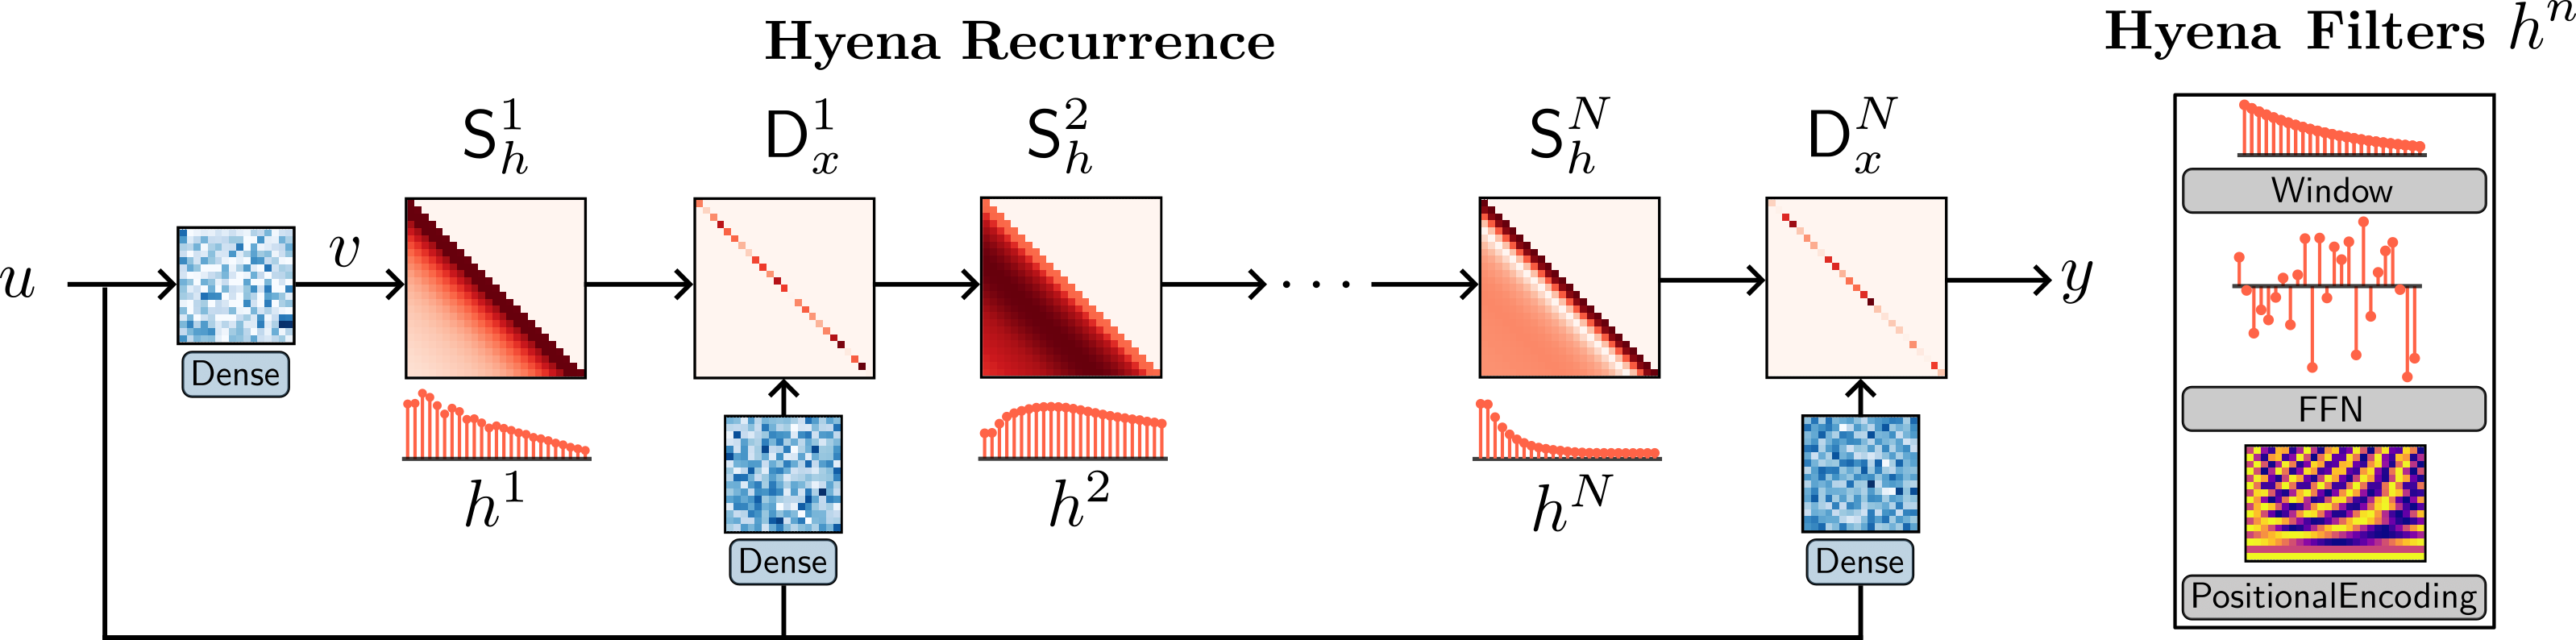
\includegraphics[width=\linewidth]{figures/hyena.png}
    \vspace{-2mm}
    \caption{The ${\sf Hyena}$ operator is defined as a recurrence of two efficient subquadratic primitives: an implicit long convolution $h$ (i.e. {\sf Hyena} filters parameterized by a feed-forward network) and multiplicative element-wise gating of the (projected) input. The depth of the recurrence specifies the size of the operator. {\sf Hyena} can equivalently be expressed as a multiplication with \textit{data-controlled} (conditioned by the input $u$) diagonal matrices $\sD_x$ and Toeplitz matrices $\sS_h$. In addition, {\sf Hyena} exhibits sublinear parameter scaling (in sequence length) and unrestricted context, similar to attention, while having lower time complexity.}
    \label{arch}
\end{figure*}
%

{\centering
\textit{Are there subquadratic operators that can match the quality of attention at scale?}\par}

\vspace{0.5cm}
% 

We obtain a positive answer based on a composition of efficient subquadratic primitives, such as \textit{element-wise multiplication} (gating) and \textit{long convolutions} i.e., convolutions with filter sizes as long as the input. We rely on a set of targeted reasoning tasks, grounded in recent work on \textit{mechanistic interpretability} \citep{elhage2021mathematical,power2022grokking,olsson2022context,zhang2022unveiling} such as recall and induction, to distill three properties of attention correlated with its performance and the quality gap with existing subquadratic approaches: 
%
\begin{itemize}[leftmargin=0.1in]
    \item[$a.$] \textbf{Data control:} Attention implements an expressive \textit{data-controlled} \citep{massaroli2020dissecting} linear operator\footnote{Self-attention can be expressed as $y = \sA(k, q) v$ where $\sA$ is the \textit{attention matrix} conditioned by linear projections $k, q$ of the input and multiplied by $v$, another projection.}, encoding an entire family of linear functions in a single block.
    \item[$b.$] \textbf{Sublinear parameter scaling:} Parameter counts of attention layers are decoupled from sequence length, allowing Transformers to allocate more parameters elsewhere e.g., the \textit{feed-forward neural networks} ({$\sf FFN$s}) between attention layers.
    \item[$c.$] \textbf{Unrestricted context:} For a given input, attention has an unrestricted context i.e., it can approximate dependencies between any two inputs, without arbitrary restrictions such as locality (except in cases using masking such as autoregressive models).
\end{itemize}
%
\paragraph{The ${\sf Hyena}$ hierarchy}
%
Guided by these findings, we introduce the ${\sf Hyena}$ hierarchy, an operator defined by a recurrence of two efficient subquadratic primitives: \textbf{a long convolution and element-wise multiplicative gating} (see Figure \ref{arch}). A specified depth (i.e., number of steps) of the recurrence controls the size of the operator. For short recurrences, existing models are recovered as special cases \citep{mehta2022long,dao2022hungry}. By mapping each step in the ${\sf Hyena}$ recurrence to its corresponding matrix form, we reveal ${\sf Hyena}$ operators to be equivalently defined as a decomposition of a \textit{data-controlled} matrix i.e., a matrix whose entries are functions of the input. Furthermore, we show how ${\sf Hyena}$ operators can be evaluated efficiently without materializing the full matrix, by leveraging fast convolution algorithms \citep{selesnick2017fast}. Empirically, ${\sf Hyena}$ operators are able to significantly shrink the quality gap with attention at scale, reaching similar perplexity and downstream performance with a smaller computational budget (Section \ref{res:lm}) and \textbf{without hybridization} of attention.
%

\paragraph{Narrowing the capabilities gap}
%
The design of {\sf Hyena} is motivated by a quality gap between standard dense attention and alternative subquadratic operators, which we identify by focusing on reasoning tasks correlated with language modeling performance at scale. We extend the suite of basic mechanistic interpretability benchmarks (\textit{induction} and \textit{recall}) with additional tasks that probe how quickly model performance degrades when task complexity increases (e.g. vocabulary size grows). In addition, we investigate the optimal parameterization of long convolutions in ${\sf Hyena}$. In the most challenging settings with hundreds of thousands of tokens, our implicit parameterization scheme improves over other operators leveraging state spaces \citep{gu2021efficiently}, frequency-domain parametrizations \citep{li2020fourier}, or standard convolutions by over $50\%$ accuracy.
%
\paragraph{Scaling in language and vision}
%
Next, we aim to verify whether rankings in our reasoning benchmark suite are predictive of quality at scale. We test ${\sf Hyena}$ on autoregressive language modeling at the sub-billion parameter scale, setting a new state-of-the-art for dense-attention-free architectures in standard datasets ({\sc WikiText103} and {\sc The Pile}) and matching Transformer quality. On the {\sc The Pile} at the $335$M parameter scale, we match Transformer perplexity with a $20\%$ reduction in the total count of \textit{floating point operations} (FLOPs). As an extension, we investigate the generality of ${\sf Hyena}$ operators by testing on large-scale image recognition, replacing attention in the Vision Transformer (ViT) \citep{dosovitskiy2020image}. In image classification, ${\sf Hyena}$ is able to match attention in accuracy when training on ImageNet-1k from scratch.
%
\paragraph{Toward much longer context}
%
Finally, we benchmark the efficiency of ${\sf Hyena}$ on long sequences. We measure $5$x speedups over dense self-attention at length $8192$ -- $2$x over highly optimized FlashAttention\footnote{FlashAttention is already 2-4x faster than a standard attention implementation in PyTorch.} \citep{dao2022flashattention} -- and $100$x speedup over FlashAttention at sequence lengths of $64$k, where standard attention implementation in PyTorch runs out of memory. 
\section{Related Work}
\subsection{Diffusion Model}
%
In the realm of generative models, diffusion models \cite{ho2020denoising, sohl2015deep} have become foundational due to their exceptional ability to produce high-quality and diverse outputs. Initially developed with the U-Net architecture, these models have demonstrated impressive performance in image and video generation \cite{ramesh2022hierarchical, rombach2022high, ho2022video, saharia2022photorealistic, wei2024dreamvideo, wei2024dreamvideo2, wang2023modelscope, chen2023videocrafter1, chen2024videocrafter2}. 
%

However, the scalability of U-Net-based diffusion models is inherently constrained, posing challenges for applications requiring larger model capacities for enhanced performance. To address this limitation, Diffusion transformers (DiT) \cite{peebles2023scalable} represent a significant advancement. By utilizing the scalable architecture of transformers \cite{vaswani2017attention}, DiT provides an effective means to increase model capacity.
%
A notable achievement in this field is the advancement in generating long videos through the large-scale training of Sora \cite{Sora}, which employs a transformer-based Diffusion architecture for comprehensive simulations of the physical world. This underscores the considerable impact of scaling transformer-based Diffusion models.
%
An increasing number of studies have adopted the Diffusion transformer as the noise estimation network~\cite{chen2023pixart, chen2024pixart, Open-Sora, Open-Sora-Plan, ma2024latte, yang2024cogvideox}.

\subsection{Diffusion Model Acceleration}
%
Despite the notable performance of Diffusion models in image and video synthesis, their significant inference costs hinder practical applications. Efforts to accelerate Diffusion model inference fall into two primary categories. First, techniques such as DDIM~\cite{song2020denoising} allow for fewer sampling steps without sacrificing quality. Additional research has focused on efficient ODE or SDE solvers~\cite{song2019generative, jolicoeur2021gotta, lu2022dpm, karras2022elucidating, lu2022dpm++}, using pseudo numerical methods for faster sampling. Second, approaches include distillation~\cite{salimans2022progressive, wang2023videolcm}, quantization~\cite{li2024q, he2024ptqd, so2024temporal, shang2023post}, and distributed inference~\cite{li2024distrifusion} are employed to reduce the workload and inference time.  

However, these methods often demand additional resources for fine-tuning or optimization. Some training-free approaches~\cite{bolya2023token, wang2024attention} streamline the sampling process by reducing input tokens, thereby eliminating redundancy in image synthesis. Other methods reuse intermediate features between successive timesteps to avoid redundant computations~\cite{wimbauer2024cache, so2023frdiff, zhang2024cross}. DeepCache~\cite{xu2018deepcache} and Faster Diffusion~\cite{li2023faster} utilize feature caching to modify the UNet Diffusion, thus enhancing acceleration. FORA~\cite{selvaraju2024fora} and $\triangle$-DiT~\cite{chen2024delta} adapts this mechanism to DiT by caching residuals between attention layers. PAB~\cite{zhao2024real} caches and broadcasts intermediate features at various timestep intervals based on different attention block characteristics for video synthesis. While these methods have improved Diffusion efficiency, enhancements for DiT in visual synthesis remain limited.
\section{Model Training}\label{sec3.model_training}




\subsection{Model Architecture}\label{sec3.1}

We opt to extend the Mistral model architecture~\cite{jiang2023mistral7b} due to its ability to achieve high performance while maintaining efficient inference speeds. The original Mistral 7B model demonstrates superior performance compared to multiple 7B language models and even outperforms larger models on various evaluation benchmarks. Notably, it surpasses the LLaMA 34B model~\cite{roziere2023code} in tasks such as mathematics and code generation.

 

\begin{wraptable}{r}{4cm}
\vspace{-12pt}\caption{Parameter setting.}\label{wrap-tab:1}
%\begin{table}[]
\begin{tabular}{l|l}
\hline
Parameter    & Value \\ \hline
n\_layers    & 36    \\
dim          & 4096  \\
head\_dim    & 128   \\
hidden\_dim  & 14336 \\
n\_heads     & 32    \\
n\_kv\_heads & 8     \\
 \hline
\end{tabular}
%\end{table}
\end{wraptable} 
The original Mistral model leverages grouped-query attention (GQA)\cite{ainslie2023gqa} and sliding window attention (SWA)\cite{beltagy2020longformer}. GQA reduces memory requirements during decoding, allowing for larger batch sizes and higher throughput, and it significantly accelerates inference speed—an essential factor in real-time applications. Meanwhile, SWA effectively handles long sequences without incurring substantial computational overhead. By incorporating these techniques, the model achieves significant improvements in performance and efficiency, which we have adopted in our extended model.



Building upon the original Mistral model, which consists of 32 blocks, we have extended the architecture to 36 blocks. Furthermore, we also employ GQA to partition the query heads into multiple groups, each sharing a single key head and value head. This approach interpolates between multi-query attention (MQA) and multi-head attention (MHA) in large language models, striking a balance between the computational speed of MQA and the representational quality of MHA, thereby providing a favorable trade-off. Additionally, our model incorporates a rolling buffer cache with a fixed attention span, effectively limiting cache size and preventing excessive memory usage when processing long sequences.




\subsection{Training Data}\label{sec3.3}

Data are fundamental to the pre-training of LLMs. Preparing such training data requires careful consideration of multiple challenges, including handling sensitive information, ensuring comprehensive knowledge coverage, and achieving higher efficiency with improved data quality. 

In this section, we detail the processes of preparing textual data from general domains and coding data related to programming languages.




\subsubsection{Text Data}

We use a mix of data from SlimPajama \cite{cerebras2023slimpajama} and DCLM-BASELINE \cite{li2024datacomp} as our text training data.

During the training of LLaMA, it was demonstrated that the performance of a 7B model continues to improve even after being trained on more than 1T tokens \cite{touvron2023llama}. Given the outstanding performance of LLaMA, its data collection methodology was rapidly replicated, leading to the release of RedPajama, an open-source dataset containing 1.2 trillion tokens \cite{weber2024redpajama}.


However, subsequent analyses reveal a significant limitation: some corpora within RedPajama contain a large percentage of duplicate content. The deduplication guidelines in RedPajama operate only within individual data sources, leaving inter-source duplicates largely unaddressed. To improve data quality and training efficiency, SlimPajama\footnote{https://huggingface.co/datasets/cerebras/SlimPajama-627B} was developed as a refined iteration of RedPajama, offering a cleaned and extensively deduplicated version \cite{cerebras2023slimpajama}.



SlimPajama implements a rigorous two-stage preprocessing pipeline to enhance data quality. In the first stage, short and low-quality documents are removed from RedPajama. Specifically, documents that have fewer than 200 characters after removing punctuation, space symbols, newlines, and tabs are filtered out, as these documents typically contain only metadata and lack useful information. As a result of this step, 1.86\% of RedPajama documents are eliminated.



The second step involves removing duplicate data, as deduplication enhances training efficiency and reduces memorization, thereby decreasing the likelihood of generating text solely by recalling training data \cite{penedo2023refinedweb, abbas2023semdedup, face2023, lee2021deduplicating, holtzman2019curious}. To perform deduplication, document signatures are created using pre-processed, lower-cased 13-grams. Subsequently, MinHashLSH~\cite{leskovec2014mining} is employed to identify and eliminate duplicates based on a Jaccard similarity threshold of 0.8. Deduplication is performed both within and across data sources. Overall, by pruning 49.6\% of the bytes from the RedPajama dataset, the 627B-token SlimPajama dataset is obtained.




Additionally, we utilize the DCLM-BASELINE \cite{li2024datacomp} dataset\footnote{https://huggingface.co/datasets/mlfoundations/dclm-baseline-1.0}, which is derived from CommonCrawl, a web-crawled dataset \cite{patel2020introduction}. The construction of DCLM-BASELINE involves several steps. First, resiliparse is employed to extract text from CommonCrawl. Second, deduplication is performed using MinHash~\cite{broder1997resemblance} within a suffix array pipeline \cite{fineweb2024, lee2021deduplicating} and near-duplicate Bloom filtering, which enhances the exact document and paragraph deduplication scheme \cite{soldaini2024dolma}. Third, recent studies \cite{brandfonbrener2024color, soldaini2024dolma, fang2023data} demonstrate that utilizing learnable models as quality filters leads to downstream performance improvements. Consequently, DCLM-BASELINE applies a fastText OH-2.5 combined with an ELI5 classifier score to retain the top 10\% of documents.



\subsubsection{Coding Data}

Programming is crucial for LLMs to support various downstream tasks, such as code completion from natural language descriptions, documentation generation for individual functions, and auto-completion of code snippets. Furthermore, as code is generally better structured and organized than natural language, training on code data may improve the LLM reasoning capabilities \cite{groeneveld2024olmo}. Therefore, We use part of the-stack-dedup \cite{kocetkov2022stack} dataset\footnote{https://huggingface.co/datasets/bigcode/the-stack-dedup} during the pretraining.

The Stack comprises more than 6TB of permissively-licensed source code files across 358 programming languages~\cite{kocetkov2022stack}. This carefully curated resource was designed to enhance the code generation capabilities of LLMs. It facilitates the synthesis of programs by code-generating AI systems from both natural language descriptions and existing code snippets.


To construct the Stack dataset, 220.92 million active GitHub repositories were collected from event archives published between 2015 and 2022 on GHArchive. Of these repositories, only 137.36 million were publicly accessible on GitHub, resulting in 51.76 billion downloaded files. After initial filtering, 5.28 billion unique files were identified, with an uncompressed size of 92.36 TB.



To ensure data quality, near-deduplication was implemented within the preprocessing pipeline in addition to exact deduplication. Specifically, MinHash with 256 permutations was computed for all documents, and Locality Sensitive Hashing was employed to identify clusters of duplicates. Within these clusters, Jaccard similarities were calculated to detect near-duplicates using a similarity threshold of 0.85. Approximately 40\% of permissively licensed files were identified as (near-)duplicates and subsequently removed.




\subsubsection{Capability Enhancement}

LLMs are expected to demonstrate capabilities such as reasoning, mathematical problem-solving, and knowledge memorizing. However, a significant challenge lies in that, in the pre-training process, high-quality capability-related data is sparsely distributed in the entire corpus, and thereby it is difficult for models to be proficient at these above-mentioned capabilities. Previous research, such as work on Qwen~\cite{bai2023qwen}, GLM-130B~\cite{zeng2023glmb}, Nemotron-4~\cite{parmar2024nemotron}, has tried to incorporate instruction-based or high-quality data during the pre-training stage to enhance these abilities. In our study, we collect open-source data from HuggingFace, primarily utilizing the training datasets of various evaluation benchmarks such as MMLU \cite{hendrycks2021measuringmassivemultitasklanguage} and HellaSwag \cite{zellers2019hellaswag}. These data are used experimentally to investigate the relationship between high-quality, capability-focused training data and model performance.


\subsection{Training Configuration}

The total number of tokens used for pre-training our Moxin-7B model is over 2T, and the pre-training process consists of three phases. In the first phase, we use pre-training corpora with the context length of 2k. In the second phase, we use pre-training corpora with the context length of 4k. In the third phase, we utilize the capability-specific enhancement data. We provide the model performance with only the first two phases and also with all three phases to validate the performance of the third phase. 

We use Colossal-AI \cite{li2023colossal} as our training framework. Colossal-AI is a unified deep learning system that provides the fullest set of acceleration techniques for the AI community. With its modular design, ColossalAI allows for a free combination of these techniques to achieve the best training speedup. Colossal-AI's optimized parallelism and heterogeneous training methods are employed to achieve superior system performance compared to baseline systems. These methods are provided through user-friendly APIs, requiring minimal code modifications.

  
During training, AdamW \cite{loshchilov2017decoupled} with $\beta_1 = 0.9$, $\beta_2 = 0.95$, $\epsilon = 1e^{-8}$ and weight decay = 0.1 is used to optimize the model. We use the cosine learning rate decay and the learning rate decays to 10\% of its maximum.  Learning Rate is set to $2e^{-6}$. 

\subsection{Alignment}


Following the pre-training phase, we fine-tune the model into a helpful and harmless AI assistant.
In our Alignment stage, we mainly use supervised fine-tuning (SFT), during which we fine-tune the model to follow diverse human instructions by high-quality instruction data. We use the Tulu v2 dataset \cite{ivison2023camels} for instruction tuning. The dataset consists of a mix of FLAN, Open Assistant 1, ShareGPT, GPT4-Alpaca, LIMA, and so on. 

\subsection{Long-Context}\label{sec3.4}

To deal with the long-context problem, our model leverages grouped-query attention (GQA)~\cite{ainslie2023gqa}, sliding window attention (SWA)~\cite{beltagy2020longformer}, and Rolling Buffer Cache \cite{jiang2023mistral7b}. GQA reduces the memory requirement during decoding, allowing for higher batch sizes hence higher throughput. 

Besides, SWA can handle longer sequences more effectively at a reduced computational cost, thereby alleviating a common limitation in LLMs. SWA exploits the stacked layers of a transformer to attend information beyond the window size $W$. 
At the last layer, with SWA, using a window size of $W = 4096$, we have a theoretical attention span of approximately $14K$ tokens or above. 


Our model adopts Rolling Buffer Cache which limits the cache size using a rolling buffer cache with a fixed attention span. The cache has a fixed size of $W$, and the keys and values for the timestep $i$ are stored in position $i$ mod $W$ of the cache. As a result, when the position $i$ is larger than $W$, past values in the cache are overwritten, and the size of the cache stops increasing. On a sequence length of $32k$ tokens, this reduces the cache memory usage by 8$\times$, without impacting the model quality.

With the above techniques, our model can support $32K$ context length with fast inference and low memory cost.

\section{Evaluation}\label{sec4.evaluation}


We conducted comprehensive performance comparisons against leading language models of comparable scale, including Mistral-7B \cite{jiang2023mistral7b}, LLaMA 2-7B \cite{touvron2023llama}, Gemma-7B \cite{team2024gemma}, and Qwen v2-7B \cite{yang2024qwen2}. These models were selected based on their demonstrated excellence within the 7B or 8B category and represent diverse development approaches from various research organizations worldwide. To ensure a robust evaluation, we re-run all benchmarks with the same evaluation pipeline for fair comparisons. Specifically, we use lm-evaluation-harness \cite{lmevaluationharness} and opencompass \cite{open_compass} for evaluation.

Lm-evaluation-harness provides a unified framework to test generative language models on a large number of different evaluation tasks. It supports over 60 standard academic benchmarks for LLMs, with hundreds of subtasks and variants implemented.
This framework is versatile as it extends to models implemented through various architectures, including transformers (including quantization via AutoGPTQ~\cite{AutoGPTQ}), GPT-NeoX~\cite{black2022gpt}, and Megatron-DeepSpeed~\cite{song2023deepspeed4science}, all unified through a flexible, tokenization-agnostic interface.
The framework is reliable, as evidenced by serving as the backend for HuggingFace's popular Open LLM Leaderboard and being utilized by dozens of organizations, including NVIDIA, Cohere, BigScience, BigCode, Nous Research, and Mosaic ML. 

To complement, we also employed openCompass. This framework performs an in-depth and holistic assessment of large language models structured around eight fundamental dimensions of language model capabilities: language comprehension, knowledge precision, logical deduction, creative ideation, mathematical problem-solving, programming proficiency, extended text analysis, and intelligent agent engagement.



\subsection{Evaluation Tasks}\label{sec4.1}

We evaluate the model performance on various tasks below.


\begin{itemize}
\item AI2 Reasoning Challenge (ARC)~\cite{allenai:arc} - a set of genuine grade-school level, multiple-choice science questions, assembled to encourage research in advanced question-answering. The dataset is partitioned into a Challenge Set (ARC-C) and an Easy Set (ARC-E), where the former contains only questions answered incorrectly by both a retrieval-based algorithm and a word co-occurrence algorithm.
\item HellaSwag~\cite{zellers2019hellaswag} - a test of commonsense natural language inference, which is easy for humans (~95\%) but challenging for SOTA models. It consists of 70,000 multiple-choice questions. Each question presents a scenario followed by four possible outcomes, asking the model to select the most reasonable conclusion.
\item MMLU~\cite{van2024ai} - a test to measure a text model's multitask accuracy. The test covers 57 tasks, including elementary mathematics, US history, computer science, law, etc.
\item Winogrande~\cite{sakaguchi2021winogrande} - an adversarial and difficult Winograd benchmark at scale, for commonsense reasoning. It contains 44,000 multiple-choice questions with two options each. It requires the model to choose the appropriate entity word for the pronoun in the descriptive text based on the scenario.
\item PIQA~\cite{bisk2019piqareasoningphysicalcommonsense} -   the task of physical commonsense reasoning and a corresponding benchmark dataset Physical Interaction: Question Answering (PIQA). Physical commonsense knowledge is a major challenge on the road to true AI-completeness, including robots that interact with the world and understand natural language. PIQA focuses on everyday situations with a preference for atypical solutions. 
\end{itemize}




\subsection{Evaluation Results}\label{sec4.2}


We name the initial model as Moxin-7B-original, which presents the foundation model before fine-tuning on the training data of the evaluation datasets. After subsequent partial fine-tuning of Moxin-7B-original on the training data of the evaluation datasets, we developed Moxin-7B-finetuned, enabling direct assessment of how targeted fine-tuning affects model performance. 





\subsubsection{Zero-Shot Evaluation}

We report the result of base models for zero-shot evaluation in Table \ref{tab:2}. The tasks are listed below. After training with the training data of evaluation tasks, our Moxin-7B-finetuned can achieve superior performance compared with state-of-the-art (SOTA) baselines. This significant increase from the base model demonstrates the effectiveness of our fine-tuning approach. The improved performance is particularly notable on complex reasoning tasks like PIQA, where the score increased from 78.07\% to 82.24\%, matching or exceeding several leading models.
Consequently, our models emerge as an excellent candidate for real-world applications. 
\begin{itemize}
\item AI2 Reasoning Challenge (0-shot)
\item AI2 Reasoning Easy (0-shot)
\item HellaSwag (0-shot)
\item PIQA (0-shot)
\item Winogrande (0-shot)
\end{itemize}

\scalebox{1.04}{
\begin{threeparttable}[t]
\caption{Performance comparison for various models in zero-shot evaluation.}
\begin{tabular}{c|ccccc|c}
\hline
Models                & HellaSwag & WinoGrade & PIQA  & ARC-E & ARC-C & Ave \\ \hline
Mistral - 7B       & 80.39     & 73.4      & 82.15 & 78.28 & 52.22 & 73.29   \\
LLaMA 2 - 7B          & 75.99     & 69.06     & 79.11 & 74.54 & 46.42 & 69.02   \\
LLaMA 2 - 13B         & 79.37     & 72.22     & 80.52 & 77.4  & 49.06 & 71.71   \\
LLaMA 3.1 - 8B        & 78.92     & 74.19     & 81.12 & 81.06 & 53.67 & 73.79   \\
gemma - 7b            & 80.45     & 73.72     & 80.9  & 79.97 & 54.1  & 73.83   \\
Qwen v2 - 7B          & 78.9      & 72.38     & 79.98 & 74.71 & 50.09 & 71.21   \\
internlm2.5 - 7b      & 79.14     & 77.9      & 80.52 & 76.16 & 51.37 & 73.02   \\
Baichuan2 - 7B        & 72.25     & 67.17     & 77.26 & 72.98 & 42.15 & 66.36   \\
Yi-1.5-9B             & 77.86     & 73.01     & 80.74 & 79.04 & 55.03 & 73.14   \\
deepseek - 7B         & 76.13     & 69.77     & 79.76 & 71.04 & 44.8  & 68.3    \\ \hline
Moxin - 7B - original & 72.06     & 66.31     & 78.07 & 71.47 & 48.15 & 67.21   \\
Moxin - 7B - finetune & 80.03     & 75.17     & 82.24 & 81.12 & 58.64 & 75.44   \\ \hline
\end{tabular}
\label{tab:2}
\end{threeparttable}}


\subsubsection{Few-Shot Evaluation}

Table \ref{tab:1} presents our zero-shot evaluation results across multiple benchmark tasks. The tasks and their few-show settings are listed below. Thanks to its rigorous and high-quality training corpus, our model demonstrates a remarkable competitive edge in tasks that involve language understanding and knowledge application. Our Moxin-7B-original achieves superior performance than LLaMA2-7B in this scenario. After training with the training data of evaluation tasks, our Moxin-7B-finetuned can achieve competitive performance compared with  SOTA baselines.


Consequently, our models emerge as an excellent choice for a multitude of real-world applications where the reliance on robust language comprehension and extensive knowledge is paramount.
\begin{itemize}
\item AI2 Reasoning Challenge (25-shot)
\item HellaSwag (10-shot)
\item MMLU (5-shot)
\item Winogrande (5-shot)
\end{itemize}




\scalebox{1.2}{
\begin{threeparttable}[t]
\caption{Performance comparison for various models in few-shot evaluation.}
\begin{tabular}{c|cccc|c}
\hline
model                  & ARC-C   & hellaswag & mmlu  & WinoGrade & Ave   \\ \hline
Mistral - 7B      & 57.59 & 83.25     & 62.42 & 78.77     & 70.51 \\
LLaMA 3.1 - 8B         & 54.61 & 81.95     & 65.16 & 77.35     & 69.77 \\
LLaMA 3 - 8B           & 55.46 & 82.09     & 65.29 & 77.82     & 70.17 \\
LLaMA 2 - 7B           & 49.74 & 78.94     & 45.89 & 74.27     & 62.21 \\
Qwen 2 - 7B            & 57.68 & 80.76     & 70.42 & 77.43     & 71.57 \\
gemma - 7B             & 56.48 & 82.31     & 63.02 & 78.3      & 70.03 \\
internlm2.5 - 7B       & 54.78 & 79.7      & 68.17 & 80.9      & 70.89 \\
Baichuan2 - 7B         & 47.87 & 73.89     & 54.13 & 70.8      & 61.67 \\
Yi-1.5-9B              & 58.36 & 80.36     & 69.54 & 77.53     & 71.48 \\ \hline
Moxin - 7B - original  & 53.75 & 75.46     & 59.43 & 70.32     & 64.74 \\
Moxin - 7B - finetuned & 59.47 & 83.08     & 60.97 & 78.69     & 70.55 \\ \hline
\end{tabular}
\label{tab:1}
\end{threeparttable}}





\subsection{Alignment Evaluation}  

\begin{wraptable}{r}{5.2cm}
\vspace{-5pt}\caption{Performance  for various chat models.}\label{tab:4}
\begin{tabular}{c|c}
\hline
Model                   & MTbench       \\ \hline
\textbf{Moxin Chat 7B} & \textbf{6.42} \\
Llama 2 Chat 13B         & 6.65          \\
Vicuna 13B              & 6.57          \\
Llama 2 Chat 7B          & 6.27          \\
Vicuna 7B               & 6.17          \\
Alpaca 13B              & 4.53          \\
\hline
\end{tabular}
\end{wraptable}
We evaluate the alignment performance on MTBench \cite{zheng2023judging}. 
It is a two-round conversation dataset with 80 questions. It covers eight dimensions (reasoning, roleplay, math, coding, writing, humanities, STEM, and information extraction) with 10 questions for each dimension. The model needs to answer the first question and then refine its previous response following additional specific instructions.  We use GPT-4 as a judge model to provide scores  (between 1-10) for the quality of responses. Our Moxin-7B-chat achieves superior performance on MTbench compared with baselines, as shown in Table~\ref{tab:4}. 


\subsection{Generation Examples}  
We demonstrate some text generation examples from our Moxin Chat 7B and Llama2 Chat 7B in Table \ref{tab:E1} and \ref{tab:E2}.


\begin{center}
\begin{threeparttable}[]

\scalebox{0.7}{
\begin{tabular}{l|l}
\hline
               & Example 1                                                                                                                                                                                                                                                                                                                                                                                                                                                                                                                                                                                                                                                                                                                                                                                                                                                                                                                                                                                                                                                                                                                                                                                                                                                                                                                                                                                                                                                                                                                                                                                                                                                                                                                                                                                                                                                                                                                                                                                                                                                                                                                                                                                                                                                                                                                                                                                                                                                                                                                                                                                                                                                                                                                                                                                                                                                                                                                                                                                                                                                                                                                                                                                                                                                                                                                    \\ \hline
Moxin Chat 7B  & \begin{tabular}[c]{@{}l@{}}Can you explain the concept of regularization in machine learning? \\ \\ Regularization is a technique used in machine learning to prevent overfitting by introducing a penalty \\ term in the loss function. The idea behind regularization is to encourage simpler models that are easier to \\ interpret and generalize better to new data. \\ \\ There are two main types of regularization: \\ 1. L1 regularization: also known as Lasso regularization, this method adds a penalty term to the loss \\ function that is proportional to the absolute value of the coefficients in the model. This encourages \\ sparsity, meaning that some coefficients may be exactly zero, which simplifies the model and makes it \\ easier to interpret. \\ 2. L2 regularization: also known as Ridge regularization, this method adds a penalty term to the loss \\ function that is proportional to the square of the coefficients in the model. This encourages shrinkage, \\ meaning that the coefficients are pulled closer to zero, which simplifies the model and reduces the \\ variance of the model estimates. \\ \\ Regularization can be used in various machine learning models, including linear regression, logistic \\ regression, and neural networks. It is often used in conjunction with other techniques such as cross-\\ validation to find the optimal hyperparameters that balance the bias-variance tradeoff and prevent \\ overfitting.\end{tabular}                                                                                                                                                                                                                                                                                                                                                                                                                                                                                                                                                                                                                                                                                                                                                                                                                                                                                                                                                                                                                                                                                                                                                                                                                                                                                                                                                                                                                                                                                                                                                                                                                                                                                                                                                                                                                         \\ \hline
Llama2 Chat 7B & \begin{tabular}[c]{@{}l@{}}Can you explain the concept of regularization in machine learning? \\ \\ Regularization is a technique used in machine learning to prevent overfitting. It involves adding a \\ penalty term to the loss function to discourage large values of the model's weights. \\ \\ There are several types of regularization, including: \\ 1. L1 regularization (Lasso): This adds a penalty term to the loss function that is proportional to the \\ absolute value of the model's weights. This encourages the model to have smaller weights, which can \\ help prevent overfitting. \\ 2. L2 regularization (Ridge): This adds a penalty term to the loss function that is proportional to the \\ square of the model's weights. This also encourages the model to have smaller weights, but it can lead \\ to some weights being set to zero, which can result in a simpler model. \\ 3. Dropout regularization: This is a type of regularization that is applied during training. It involves \\ randomly setting a fraction of the model's neurons to zero during each training iteration. This helps to \\ prevent overfitting by making the model less reliant on any single neuron. 4. Early stopping: This is a \\ type of regularization that is applied during training. It involves monitoring the validation loss during \\ training and stopping the training process when the validation loss stops improving. This helps to prevent \\ overfitting by stopping the training process before the model has a chance to fit the noise in the training \\ data. \\ \\ Regularization can be applied to different layers of a neural network, such as the input layer, hidden \\ layers, or output layer. It can also be applied to different parts of a model, such as the weights, biases, or \\ activation functions. The main idea behind regularization is to add a penalty term to the loss function that \\ discourages large values of the model's weights. This helps to prevent overfitting by encouraging the \\ model to find a simpler solution that generalizes better to new data. \\ \\ Regularization can be used in conjunction with other techniques, such as cross-validation and grid search, \\ to improve the performance of a machine learning model. In summary, regularization is a technique used \\ in machine learning to prevent overfitting by adding a penalty term to the loss function. There are several \\ types of regularization, including L1, L2, dropout, and early stopping, and it can be applied to different \\ layers and parts of a model. Regularization helps to find a simpler solution that generalizes better to new \\ data and can be used in conjunction with other techniques to improve the performance of a machine \\ learning model.\end{tabular} \\ \hline
\end{tabular}}
\caption{Generation Examples.} \label{tab:E1}
\end{threeparttable}
\end{center}





\begin{center}
\begin{threeparttable}[t]
\scalebox{0.7}{
\begin{tabular}{l|l}
\hline                                                               & Example 2                                                                                                                                                                                                                                                                                                                                                                                                                                                                                                                                                                                                                                                                                                                                                                                                                                                                                                                                                                                                                                                                                                                                                                                                                                                                                                                                                                                                                                                                                                                                                                                                                                                                                                                                                                                                                                                                                                                                                                                                                                                                                                                                                                                                                                                                                                                                                                                                                                                                                                                                                                                                                                                                                                                                                                                                                                                                                                                                                                                                                                                                                                                                                                                                                                                                                                                    \\ \hline
Moxin Chat 7B  & \begin{tabular}[c]{@{}l@{}}Can you explain the concept of normalization in machine learning? \\ \\ Normalization is a technique used to scale the data before using it for training a machine learning model. \\ It is used to make the data more uniform, and to prevent it from being skewed by large or small values. \\ \\ There are several ways to normalize data, including min-max scaling, z-score normalization, and \\ logarithmic scaling. In min-max scaling, the values are scaled to a range between 0 and 1, by dividing \\ them by the maximum value in the dataset. In z-score normalization, the values are scaled to have a mean \\ of 0 and a standard deviation of 1, by subtracting the mean from each value and dividing by the standard \\ deviation. In logarithmic scaling, the values are transformed using the logarithm function, which can be \\ useful for normalizing data with a wide range of values. \\ \\ Normalization is an important step in preparing data for machine learning, as it can help to improve the \\ performance of the model by making the data more uniform and easier to analyze. It can also help to \\ prevent overfitting and improve generalization.\end{tabular}                                                                                                                                                                                                                                                                                                                                                                                                                                                                                                                                                                                                                                                                                                                                                                                                                                                                                                                                                                                                                                                                                                                                                                                                                                                                                                                                                                                                                                                                                                                                                                                                                                                                                                                                                                                                                                                                                                                                                                                                                                                                                               \\ \hline
Llama2 Chat 7B & \begin{tabular}[c]{@{}l@{}}Can you explain the concept of normalization in machine learning? \\ \\ Normalization is a technique used in machine learning to transform input data into a range of values that \\ are suitable for use in a model. The goal of normalization is to ensure that the data is on the same scale, so \\ that the model can learn meaningful relationships between the features. \\ \\ There are several types of normalization techniques, including: \\ 1. Min-max normalization: This involves scaling the data so that it falls within a specific range, usually \\ between 0 and 1. \\ 2. Standardization: This involves subtracting the mean and dividing by the standard deviation of the data, \\ so that the data has a mean of 0 and a standard deviation of 1. \\ 3. Z-score normalization: This involves subtracting the mean and dividing by the standard deviation of \\ the data, so that the data has a mean of 0 and a standard deviation of 1. \\ 4. Log transformation: This involves taking the logarithm of the data, which can help to reduce the effect \\ of extreme values in the data. \\ 5. Square root transformation: This involves taking the square root of the data, which can help to reduce \\ the effect of outliers in the data. \\ \\ Normalization is an important preprocessing step in machine learning, as it can help to improve the \\ performance of the model by reducing the effect of irrelevant features and improving the interpretability \\ of the results. \\ \\ Here are some key points to keep in mind when normalizing data for machine learning: \\ 1. Normalization can improve the performance of the model by reducing the effect of irrelevant features \\ and improving the interpretability of the results. \\ 2. There are several types of normalization techniques, including min-max normalization, standardization, \\ z-score normalization, log transformation, and square root transformation. \\ 3. The choice of normalization technique will depend on the nature of the data and the specific \\ requirements of the model. \\ 4. Normalization can be applied to both continuous and categorical data. \\ 5. It is important to normalize the data before training the model, as normalization can improve the \\ convergence of the model and reduce the risk of overfitting. \\ 6. Normalization can also be used to improve the interpretability of the results by reducing the effect of \\ irrelevant features and improving the scalability of the model. \\ 7. It is important to carefully evaluate the performance of the normalized data and consider the trade-offs \\ between different normalization techniques. \\ 8. Normalization can be applied to different features of the data, such as the input features, the target \\ variable, or the output features. \\ 9. Normalization can be used in combination with other preprocessing techniques, such as feature scaling, \\ feature selection, and data augmentation. \\ 10. Normalization is a powerful tool for improving the performance of machine learning models, but it is \\ important to carefully evaluate the performance of the normalized data and consider the trade-offs \\ between different normalization techniques.\end{tabular} \\ \hline
\end{tabular}}
\caption{Generation Examples.}
\label{tab:E2}
\end{threeparttable}
\end{center}


\vspace{-5pt}
\section{Conclusion}\label{sec:conclusion}
\vspace{-5pt}
We accelerate high-resolution diffusion models by designing deep compression autoencoders to reduce the number of tokens. We proposed two techniques: \textit{residual autoencoding} and \textit{decoupled high-resolution adaptation} to address the challenges brought by the high compression ratio. The resulting new autoencoder family \modelshort demonstrated satisfactory reconstruction accuracy with a spatial compression ratio of up to 128. \modelshort also demonstrated significant training and inference efficiency improvements when applied to latent diffusion models. 

\section*{Acknowledgements}
We thank NVIDIA for donating the DGX machines. We thank MIT-IBM Watson AI Lab, MIT and Amazon Science Hub, MIT AI Hardware Program, and National Science Foundation for supporting this research. 


\bibliographystyle{unsrt}
\bibliography{sample}

\end{document}